\section{Electrophysiological Measurement Distributions from the Experimental Literature}
\label{sec:data-sources}
Organized, publicly available electrophysiological measurements from single, biological neurons can form an optimization target.
Together, they can be used to parameterize a suite of tests against which a model is optimized.
Optimization aims to find model parameters so that electrophysiological measurements based on model simulations are as similar as possible to those observed in neurons.

\subsection{NeuroElectro}
\label{sec:neuroelectro}
One general source of such experimental measurements is The NeuroElectro Project \citep{tripathy2014neuroelectro}, which contains experimental values for 47 distinct electrophysiological measurements across 235 different neuron types.
As with most of the data discussed here, most (but not all) of these measurements were obtained from slice physiology experiments in rodents.
These measurements were programatically extracted from peer-reviewed journal articles over a $\sim20$ year period from $\sim1990-2012$,
and are made easy to access by an application programming interface (API) that NeuronUnit provides bindings to.
Importantly, the measured values--even for a single neuron type--reflect experiments done in many labs using (in some cases) variable methods.
Therefore, the mean of these values (e.g. the mean input resistance across reported Purkinje cells) averages over heterogeneity across cells within a slice, slices within an animal, animals within a lab, and labs within the field.
The sample size for one measure (e.g. input resistance) may be larger than for another (e.g. resting potential) meaning that these measures may reflect different subsets of experiments.
With those caveats in mind, NeuroElectro remains the most direct way to get a large number of optimization-constraining data values for most neuron types.

In order to verify that the data from NeuroElectro was plausible and was being captured correctly for the purposes of the work in this thesis, I used the API along with a batch visualization pipeline to visualize the distributions of electrophysiological measurements and inspect them for a) quality control and b) evidence of multimodality.
Multimodality, meaning multiple peaks in the histogram of a single measurement type for a single cell, could be evidence of a physiological heterogeneity not easily explained by random measurement error.
Two peaks in the histogram, for example, could result from two distinct subclasses of a single nominal neuron type, each with its own (narrower) distribution of the same measurement.
In some instances, the mean and standard deviation alone described the measurement distributions well, as would be expected for random, normally-distributed measurements of a single cell type under reasonably consistent conditions.
These values were then ``approved" for use in model-fitting.
In other cases, these conditions were not met, as exemplified in the figures below.

%\begin{comment}
%\begin{figure}
%\centering
%   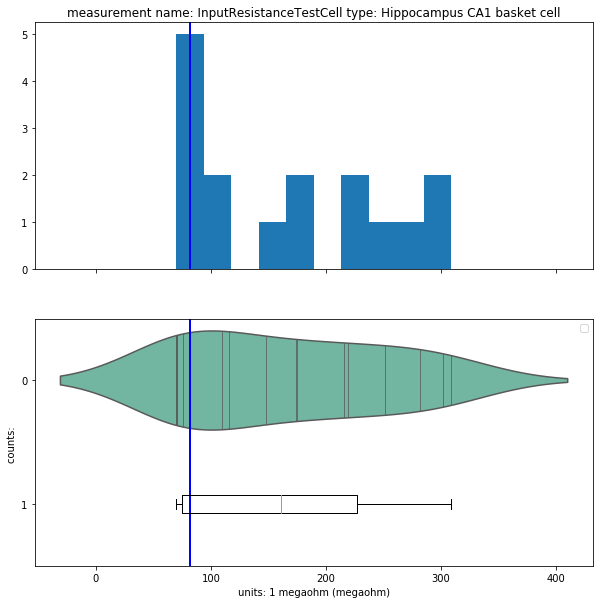
\includegraphics[scale=0.8]{notebooks_converted/needata_thesis_files/needata_thesis_5_5}
%\end{figure}

%\caption{Model parameterization of the brian2 simulator with the customization: interpolated spike height, forced to be above $0mV$}
%
%  \label{fig:sub1}
%\end{subfigure}%
%\begin{figure}
%\centering
%  \includegraphics[scale=0.8]{notebooks_converted/needata_thesis_files/needata_thesis_5_6}
%\end{figure}

%    
%    %\caption{Default model parameterization of the custom written integrator}
%  \label{fig:sub2}
%
%\begin{subfigure}
%  \centering
%      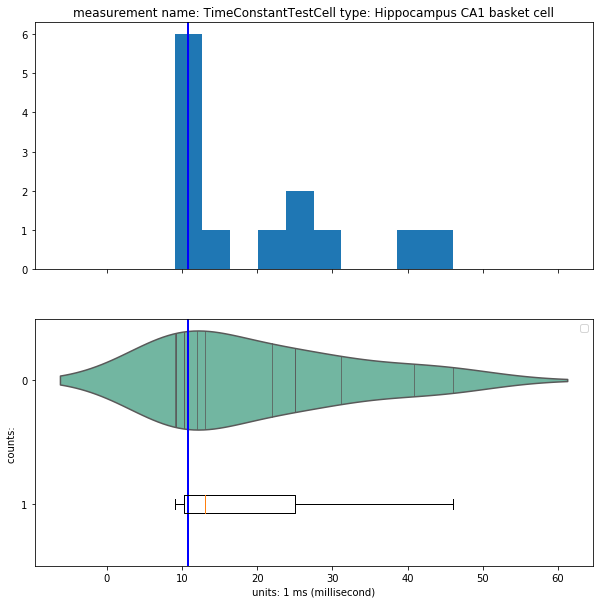
\includegraphics[scale=0.8]{notebooks_converted/needata_thesis_files/needata_thesis_5_7}
%      %\caption{Default model parameterization of the custom written integrator}
%  \label{fig:sub2}
%\end{subfigure}
%
%\caption{Comparison between two Adxaptive Exponential Implementations}
%\label{fig:test}
%\end{center}
%\end{figure}
%
%\end{comment}

%\begin{center}
%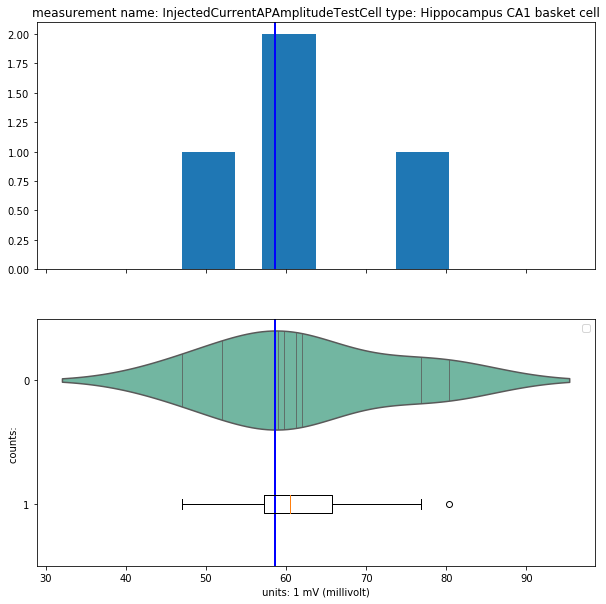
\includegraphics[width=0.7\linewidth]{notebooks_converted/needata_thesis_files/needata_thesis_5_8}
%\end{center}
%
For the majority of cell types and electrophysiological features, the distributions obtained from NeuroElectro were well-described by a normal (or log-normal) distribution.
However, I manually identified and labeled those cases where the data were not well-behaved, as these cases are likely to produce optimized models that do not reflect anything of biological relevance.

Methods for verifying that a distribution is unimodal exist \citep{maechler2013package}; however, rather than entrust this job to top-down automation, I decided to apply my own human knowledge of statistics in order to assess each distribution individually. %, because there seemed to be less opportunity to suffer from some kind of machine introduced violation of intuition. % too each  

%I achieved greater quality control through visual inspection of each case in a piece-meal manner. % manually means to do something by hand. 
I estimated that across all NeuroElectro data sampled here, about $2/3$ of distributions are well represented by a unimodal and normal distributions (e.g. Figure \ref{fig:normal-feature}).
In the remaining $1/3$, where this did not hold, I observed a small but still significant number of odd cases: highly skewed distributions (Figure \ref{fig:skewed-feature}), bimodal distributions (Figure \ref{fig:bimodal-feature}), uniform-like distributions, and distributions with insufficient samples to make any judgement.

\begin{figure} 
    \begin{center}
   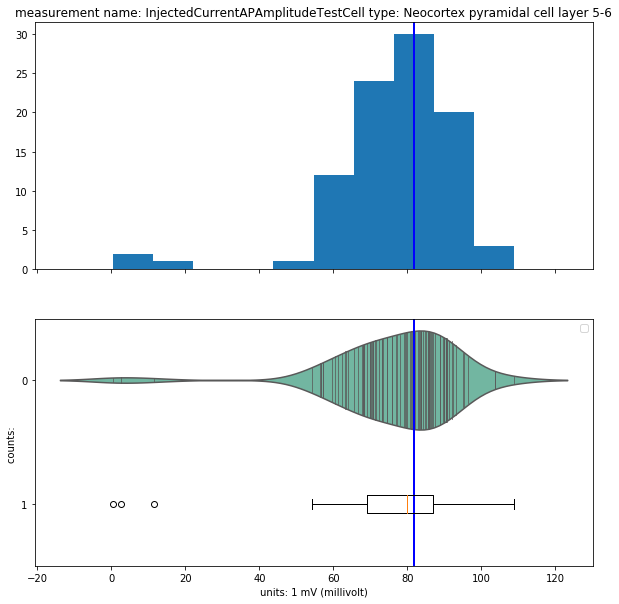
\includegraphics[scale=0.8]{figures/mean_well_served.png}
   \caption[AP Threshold Data Distribution for Layer 5 Pyramidal Cell]{\textbf{AP Threshold Data Distribution for Layer 5 Pyramidal Cell.} The majority of NeuroElectro data sets followed a normal distribution, where the mean is surrounded by a very high density of samples, which slowly thin out with increasing distance from the mean. The distribution is approximately symmetrical. Top Panel: A histogram of AP Threshold measurements from Layer 5 Pyramidal Cells; Bottom Panel: A violin plot and a box plot summarizing the same distribution. In this plot, the mean and mode are close together (a necessary condition for near-normality).
   Analagous plots were generated and inspected for all electrophysiological features computed here.}
   \label{fig:normal-feature}
    \end{center}
\end{figure}   

%\begin{figure} 
%    \begin{center}
%    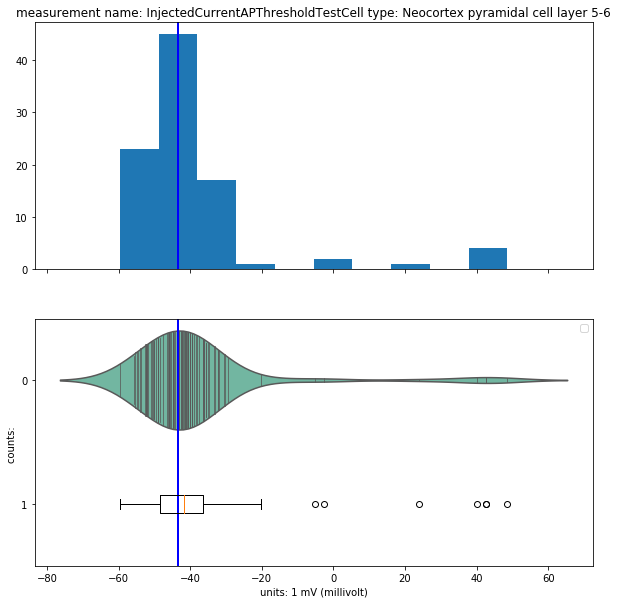
\includegraphics[scale=0.8]{figures/mean_well_served2.png}
%    \end{center}
%    \caption[AP Amplitude Data Distribution for Layer 5 Pyramidal Cell]{\textbf{AP Amplitude Data Distribution for Layer 5 Pyramidal Cell.} Same as the figure above, but for the AP Amplitude.}
%    \label{fig:normal-feature2}
%\end{figure}   
 
\begin{figure} 
    \begin{center} 
    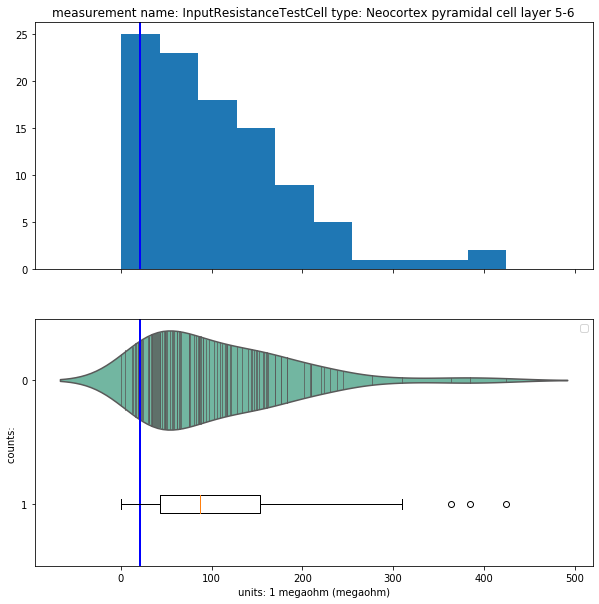
\includegraphics[scale=0.8]{figures/skewed_distribution.png}
    \end{center}
    \caption[Example of Skewed Distribution]{\textbf{Input Resistance Data Distribution for Layer 5 Pyramidal Cell.} Similar to Figure \ref{fig:normal-feature}, except for Input Resistance.
    Unlike in that figure, the distribution shows a strong skew towards higher values.
    The mean and the mode are no longer well-aligned, and therefore the mean is no longer representative of the most typical value of this feature for this neuron type.}
    \label{fig:skewed-feature}
\end{figure}   

%\begin{figure} 
%\caption[NeuroElectro data - uniform distribution]{}
%    \begin{center}
%    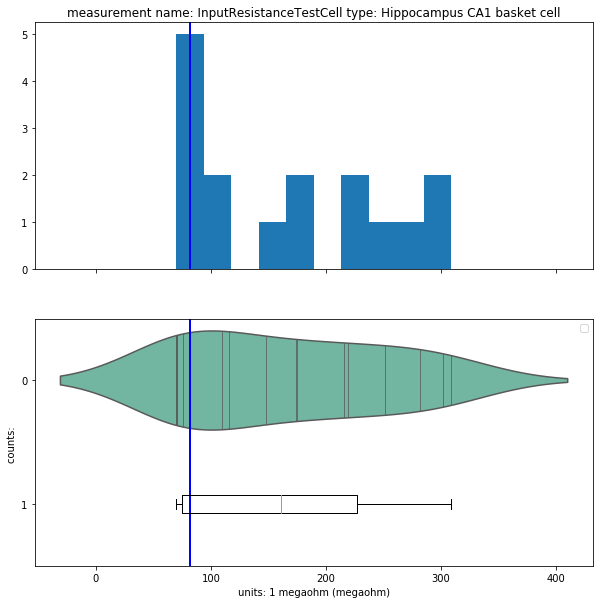
\includegraphics[scale=0.8]{figures/uniform_distribution.png}
%    \end{center}
%\end{figure}       
%%
% Neuronunit code handles under sampled neuroelectro code.
%\begin{figure} 
%\caption[NeuroElectro data - undersampled distribution]{}
%    \begin{center}
%    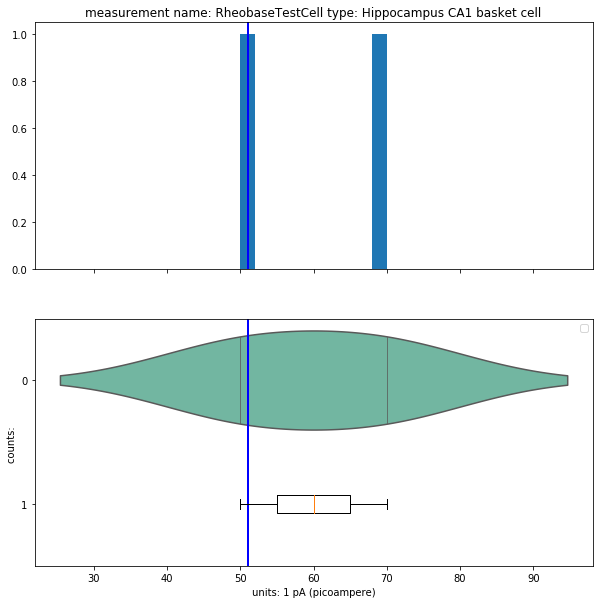
\includegraphics[scale=0.8]{figures/undersampled_distribution.png}
%    \end{center}
%\end{figure}   
%%
    
%\begin{figure} 
%    \begin{center}
%   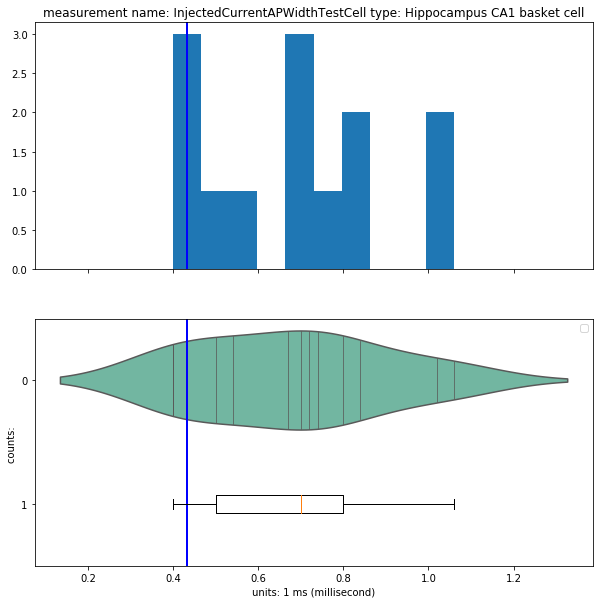
\includegraphics[scale=0.8]{chapters/notebooks_converted/needata_thesis_files/needata_thesis_5_9}
%   \caption{The Action Potential Width of the Hippocampus CA1 basket cell possibly has either an underlying uniform distribution or a multimodal distribution. Since the samples are few, the true distribution is unknown. If the distribution is uniform the gaps in the distribution, that give the histogram a multimodal appearance, as the sample size is lower enough that such gaps may only represent missing samples.}
%    \end{center}
%\end{figure}


%\begin{figure}   
%\begin{center}
%   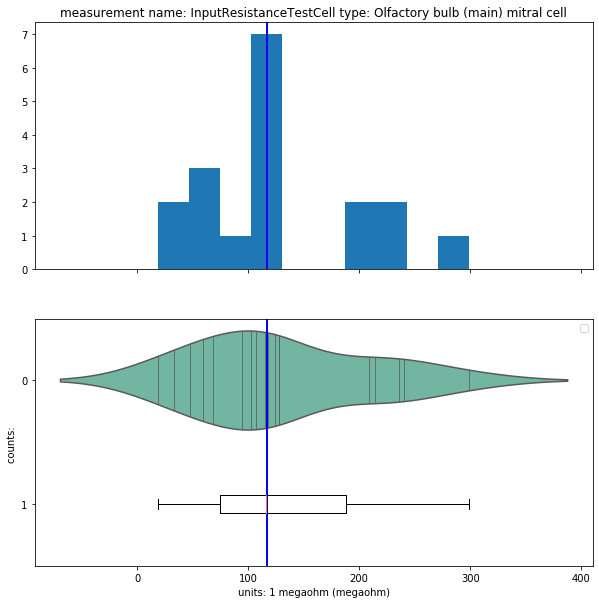
\includegraphics[scale=0.8]{chapters/notebooks_converted/needata_thesis_files/needata_thesis_5_21}
%         \caption[Input Resistance Olfactory Neuron, Perhaps Bimodal]{Input resistance of the Olfactory Mitral cell showed some tendency towards underlying bi-modal distribution, however in the second block of histogram bins, centered around $200-300pA$ only contains approximately $5$ samples. Due to a lack of samples it is also possible to conclude that the data belong to an under sampeled uniform distribution. This data set was important, as one Olfactory neuron test was constructed from this data.}
%\end{center}
%\end{figure}
   
\begin{figure}  
\begin{center}     
  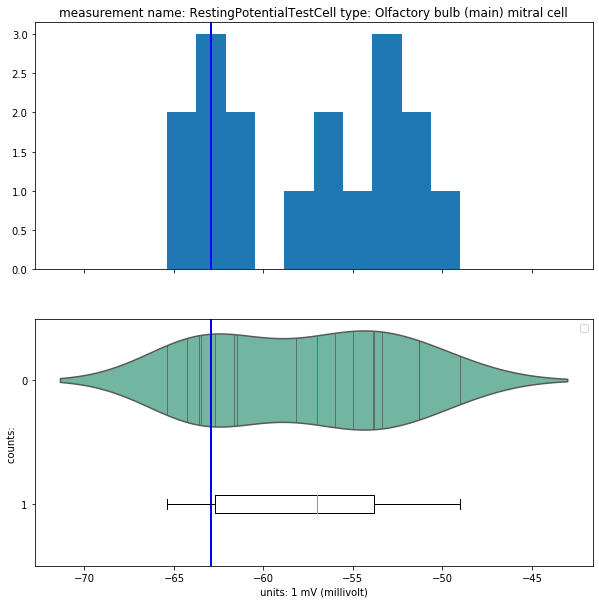
\includegraphics[scale=0.8]{chapters/notebooks_converted/needata_thesis_files/needata_thesis_5_22}
      \caption[Bi-modal Distribution for Resting Membrane Potential from Mitral Cells]{\textbf{Resting Potential Data Distribution for the Olfactory Bulb Mitral Cell.} Similar to the previous figures, but for a different cell type and electrophysiological feature.
      In this case, the distribution is clearly bimodal, with each mode containing a similar density of the data.
      Now both the mean and the median (small red line in box plot) are especially unrepresentative, lying in a region of low probabilty density.
      }
      \label{fig:bimodal-feature}
\end{center}     
\end{figure}
%%
% There are plenty of examples of bi-modal distributions in measurements from cells which are not relevant to this work.
%
%\begin{figure}
%  \centering
%  \includegraphics[scale=0.8]{chapters/notebooks_conv%erted/needata_thesis_files/needata_thesis_5_6}
%   \caption{Default model parameterization of the custom written integrator}
%  \label{fig:sub2}
%\end{figure}
%\begin{figure}
%\begin{center}
%includegraphics{chapters/notebooks_converted/needata_thesis_files/needata_thesis_5_13}
%\end{center}
%\end{figure}
    
%\begin{figure}
%\begin{center}
%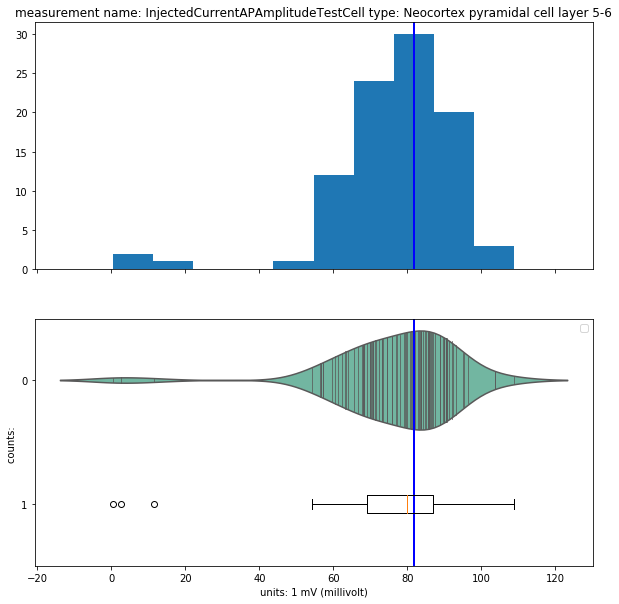
\includegraphics[width=0.7\linewidth]{chapters/notebooks_converted/needata_thesis_files/needata_thesis_5_16}
%\caption[Spike Width Measurements from Neocortical Pyramidal Neurons]{\textbf{Spike Width Measurements from Neocortical Pyramidal Neurons.} (Top Panel) Binned histogram of NeuroElectro spike width measurements from neocortical pyramidal neurons.
%The mode is denoted by the blue vertical line. The mode can be compared to the mean shown in the box plot. Often modes and means of measurements disagree.  NeuroElectro shows that a very common distribution shape is one which is possibly uniform or multi-modal. It is worth noting that a uniform distribution is not well-described by a normal distribution.}
%\label{fig:uniform-feature}
%\end{center}
%\end{figure}

%\begin{figure}
%\begin{center}
%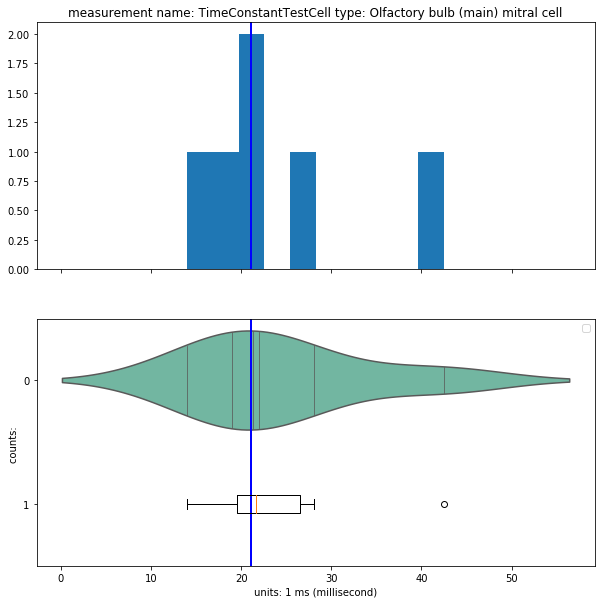
\includegraphics[scale=0.8]{chapters/notebooks_converted/needata_thesis_files/needata_thesis_5_23}
%\caption{Similar to the figure above, but for a different neuron type.}
%\label{fig:uniform-feature2}
%\end{center}
%\end{figure}

\subsection{EFEL and The Allen Institute Cell Types Database}
The Electrophysiology Feature Extraction Library (EFEL) \citep{EFEL} was developed as part of the Blue Brain Project. Although EFEL computes common spike train statistics related to spike timing, approximately 2/3rds of features extracted by EFEL pertain to spike shape, where some of these features are shown below. 
The Allen SDK comes with a very comprehensive Python-based feature extraction suite. Like EFEL, the Allen suite well-represents a large number of spike shape measurements as well as spike train statistics. 
Unfortunately, the Allen SDK feature extractor is significantly slower than EFEL, as EFEL was implemented using the very fast language $C++$. The performance cost may not be felt when dispatching single runs, but slow performance is a significant impediment to optimization. 
In optimisation, feature extraction is directly coupled to chromosome fitness calculations, and it is executed very often across the evolution of the genetic algorithm. Additionally by default, the Allen SDK feature extractor assumes that the user will apply very high sample frequency and noisy traces encoded in the NeuronData Without Borders \citep{teeters2015neurodata} standardized format. 
These traces require filtering before computing the Allen features, where significant intervention is required to turn off filtering. 
Inappropriately applying filtering to model traces causes problems, because the the lower sampling frequency intrinsic to simulated model traces is not predicted by the digital filter. Overall, the EFEL was fast enough to be useful, and its default settings were appropriate to my use case \citep{garcia2014neo}.

Data available through NeuroElectro cover a large number of cell types; however, recording conditions and measurement algorithms are heterogeneous.
It is unclear whether the distribution of measurements across such an ensemble is actually a good summary of any one individual neuron.
In order to ensure that reduced models could be optimized against data recorded exclusively from single neurons, I also used data from the Allen Institute Cell Types Database \citep{celltypes}, a project of the Allen Institute for Brain Science.
This Cell Types database consists of summary physiological, morphological, and histological data for thousands of individual neurons (across a few dozen subtypes) from mouse visual cortex, obtained using patch clamp recordings in slices.
Each experiment is done using exactly the same methods and with the same sequence of stimuli \citep{celltypes}, ensuring not only that models generated using this data are directly comparable, but that each such model is reflective of an individual neuron.

The Cell Types Database provides some limited pre-computed measures of action potential waveform characteristics. 
However, the data are not organized in a way that makes it is useful for the types of optimization and data analysis performed here.
Specifically, I require features that are computed on cell responses to current injection values that are fixed multiples of rheobase.
Additionally, the pre-computed features are thin relative to those that used for the optimizations described in the Results section.
Because raw data are available through the Cell Types API, I re-computed all necessary features from this raw data, according to the consistent standards reflected in the NeuronUnit code.

In contrast to NeuroElectro, the Cell Types database also has a great deal more information relevant to the above threshold dynamics of neurons, such as the number and pattern of action potentials they discharge in response to somatically-injected currents much larger than rheobase, or in response to non-square injected currents.
In order to exploit these, I developed several additional NeuronUnit tests using EFEL (describe later in sections \ref{sec:efel}), such as: ``time to first spike test", ``mean AP amplitude test", ``time to last spike test" and ``adaption index". In principal any feature measured in the Cell Types Data could be upgraded to a NeuronUnit test, and I created a code-generation template to accelerate this task. Effectively, code generation meant, that any EFEL feature, could be turned into a NeuronUnit test. In principle Allen tests can be generated from templates in much the same way. The final set of operational tests
were EFEL \cite{EFEL} tests that were adapted from descriptions of feature extraction in the literature and shown in Table \ref{tab:features}. 
Features are shown in Figures \ref{fig:voltage_figures} and \ref{fig:features_example}.
I also crafted additional NeuronUnit tests to supplement these including one that measures the slope of the FI curve ($FISlopeTest$) and one that measures the coefficient of variation of the ISI distribution for suprathresholds stimuli ($ISICVTest$), a measure of burstiness. 
%%
% \ref{sec:allensdk},
% Allen are features, not tests (no judge methods).
% currently, its very transient.
% Allen used to be tests, it was hard to % maintain code. 

%%%
% Tests I rewrote from scratch 
% not EFEL, was FITest, CVTest, ISITest
%%%


%\begin{figure}
%\centering
%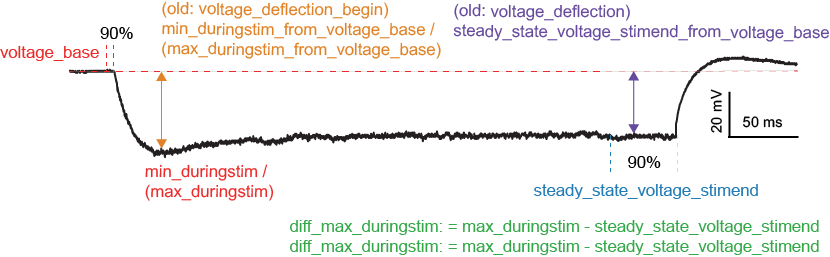
\includegraphics{figures/voltage_features.png}
%\caption[Passive Membrane Properties Measured from a Hyperpolarizing Current Stimulus]{\textbf{Passive Membrane Properties from a Hyperpolarizing Stimulus.} Applying a negative (outward, hyperpolarizing) current stimulus minimially activates voltage-dependent ion channels, making it a good method for measuring ``passive" membrane properties such as the input resistance (measured as the difference between the resting potential (red) and steady-state hyperolarization (blue).
%Nonetheless, some intrinsic conductances are activated, allowing for measurment of additional features such as the sag ratio (red trough vs blue steady state). Figure from EFEL documentation \url{https://efel.readthedocs.io/en/latest/eFeatures.html}.}
%\label{fig:voltage_figures}
%\end{figure}

\begin{figure}
\begin{center}
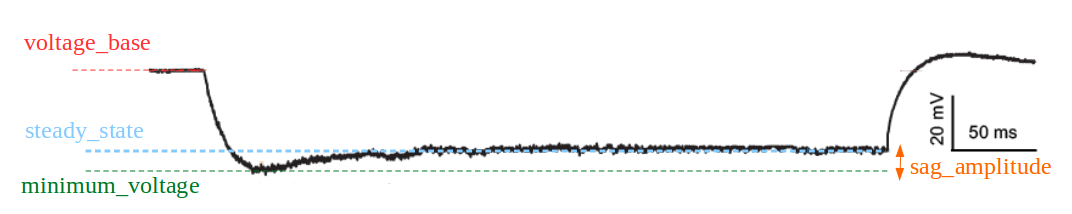
\includegraphics{figures/sag_amplitude}
\end{center}
\caption[Passive Membrane Properties Measured from a Hyperpolarizing Current Stimulus]{\textbf{Passive Membrane Properties from a Hyperpolarizing Stimulus.} Applying a negative (outward, hyperpolarizing) current stimulus minimially activates voltage-dependent ion channels, making it a good method for measuring ``passive" membrane properties such as the input resistance (measured as the difference between the resting potential (red) and steady-state hyperpolarization (green).
Nonetheless, some intrinsic conductances are activated, allowing for measurment of additional features such as the sag amplitude or ratio (green trough vs blue steady state). Figure from EFEL documentation \citep{efel-docs}.}
\label{fig:voltage_figures}
\end{figure}

\begin{figure}
\centering
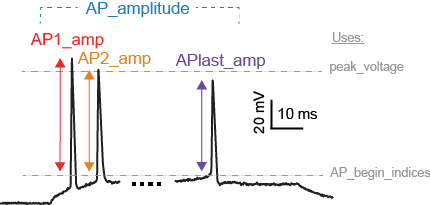
\includegraphics{figures/AP_Amplitude.png}
\caption[Action Potential Features Measured from a Depolarizing Current Stimulus]{\textbf{Action Potential Features Measured from a Depolarizing Current Stimulus.} A positive (depolarizing, inward) current of sufficiently amplitude produces one or more action poentials.
Many features can be computed from these, including their absolute amplitudes (in color), relative amplitudes, widths, thresholds, and afterhyperpolarizations (AHPs).
Additional features about their number and relative timing can also be computed (not shown).
Figure from EFEL documentation \citep{efel_documentation}.}
\label{fig:features_example}
\end{figure}



%XXXX Russell, can you list the new tests above.

These tests can be used to assess the agreement between neuron models and biological neurons on supra-threshold dynamics, largely reflected in patterns of spiking such as bursting and adaptation, but also mean spike height and mean spike width, resting membrane potential, mean trough depth, and upstroke times.

\subsection{The Blue Brain Project Neocortical Microcircuit Portal}
\label{sec:bluebrain-data}
I also made use of an additional data source, the The Blue Brain Project Neocortical Microcircuit Portal, similar in some ways to the Allen Institute Cell Types Database but reflecting measurements taken from mouse somatosensory cortex (again in patch-clamp recordings from slices).
From this dataset I exclusively used a collection of experiments from animal $B95$, which for reasons unknown yielded a tremendous amount of data \citep{ramaswamy2015neocortical}.
Conceptually, this dataset did not add anything new, but it did allow for high-quality optimized models to be produced from another brain region (somatosensory, rather than visual cortex).
These data are also linked to--and constrain--the on-going Human Brain Project effort to simulate biophysically-detailed multi-compartmental models of the same neurons (and whole neural circuits).
This means that the reduced models produced here can be compared directly to those more detailed models, or that the general NeuronUnit-driven genetic optimization framework developed here could be used to optimize detailed models which should, in principle, be similar to those produced through the larger Human Brain Project effort.
Indeed, the Human Brain Project is already a user of the SciUnit framework developed in my lab, on which NeuronUnit is based.

\begin{table}
\centering

\resizebox{\textwidth}{!}{
\begin{tabular}{|l|l|}
            \toprule
            \textbf{Test Name} & \textbf{Test Description}\\
\midrule
adaptation-index & Measures spiking fatigue in response to constant current\\
 adaptation-index2 & The same as Adaption index1, except it is used as an alternative when spikes below $0mV$ occur.   \\
time-to-first-spike & amount of time elapsed until first spike \\ mean-AP-amplitude & The average spike height in a spike train \\
spike-half-width & The width of a spike is obtained at point when spike height is half its total amplitude\\    
AHP-depth & The after hyperpolarisation depth\\
minimum-voltage & The minimum voltage\\
peak-voltage & the maximum voltage, usually a spike peak. \\
time-to-last-spike & The time of last spike onset \\
AHP-depth-abs & After Hyperpolarisation depth (absolute value).\\
all-ISI-values & All interspike interval times\\
voltage-base & minimum voltage while undergoing stimulus, often below the threshold of APs. \\
min-voltage-between-spikes & Needed because during  high frequency firing AHPs may be skipped.\\
Spikecount & Just the number of spikes that occured in the provided stimulus window\\
\bottomrule
\end{tabular}}
\caption[List of EFEL features]{14 key features identified in the EFEL \citep{EFEL} library that I impemented and encoded into NeuronUnit tests for optimization.}
\label{tab:features}
\end{table}

% There is no "NeuronUnit" data. What does this mean?
The tests which lead to the best fits in the above threshold experiments were the tests made from application of EFEL features to Allen data sources (Figure \ref{fig:voltage_figures}). The measurement type and the test type did not change between Allen Cell Types and Blue Brain Data. Only the reference data which informed comparison measurements changed. % \ref{fig:supra-threshold-tests})

Table \ref{tab:features} constitutes a summary of both NeuroElectro and Allen experimental data reports. %This data can naturally be reported in tabular form. 

%\subsection{Experimental Measurements}

\begin{table}[ht]
\centering
\resizebox{\textwidth}{!}{
\begin{tabular}{|l|l|l|l|l|l|l|l|l|}
\toprule
Test Name / Cell Type & CA1 Pyramidal & Purkinje & NCP Layer 5-6 &      Mitral Cell & 623960880 & 623893177 & 471819401 & 482493761 \\
\midrule
RheobaseTest                   &                      189.24 pA &                680.79 pA &                          213.85 pA &          NaN &        70.0 pA &       190.0 pA &       190.0 pA &        70.0 pA \\
InputResistanceTest            &                    107.08 $M\Omega$ &              142.06 $M\Omega$ &                        120.67 $M\Omega$ &  130.08 $M\Omega$ &  241.0 $M\Omega$ &  136.0 $M\Omega$ &  132.0 $M\Omega$ &  132.0 $M\Omega$ \\
TimeConstantTest               &                        24.5 ms &                      NaN &                           15.73 ms &     24.48 ms &        23.8 ms &        27.8 ms &        13.8 ms &        24.4 ms \\
CapacitanceTest                &                        89.8 pF &                620.27 pF &                          150.58 pF &    235.75 pF &            NaN &            NaN &            NaN &            NaN \\
RestingPotentialTest           &                      -65.23 mV &                -61.59 mV &                          -68.25 mV &    -58.14 mV &       -65.1 mV &       -77.0 mV &       -77.5 mV &       -71.6 mV \\
InjectedCurrentAPWidthTest     &                        1.32 ms &                  0.41 ms &                            1.21 ms &      1.61 ms &            NaN &            NaN &            NaN &            NaN \\
InjectedCurrentAPAmplitudeTest &                       86.36 mV &                 71.23 mV &                           80.44 mV &      68.4 mV &            NaN &            NaN &            NaN &            NaN \\
InjectedCurrentAPThresholdTest &                       -47.6 mV &                -46.89 mV &                          -42.74 mV &     -38.9 mV &            NaN &            NaN &            NaN &            NaN \\
FISlopeTest                         &                            NaN &                      NaN &                         0.05 Hz/pA &          NaN &     0.18 Hz/pA &     0.12 Hz/pA &     0.18 Hz/pA &     0.09 Hz/pA \\
\bottomrule
\end{tabular}}
\caption[Neuroelectro Data]{Data for 9 tests (features) across 8 cells.
The first 4 cells are specific cell types spanning several brain regions, and the corresponding data comes from neuroelectro.org.
The remaining 4 are single (cortical) cells comes from the Allen Cell Types database, and the features were directly computed using NeuronUnit tests.
``NCP" indicates neocortical pyramidal.}
\label{tab:neuroelectro-data}
\end{table}

